\documentclass[a4paper]{article}
\usepackage[utf8]{inputenc}
\usepackage{amsmath}
\usepackage{graphicx}
\usepackage{caption}
\usepackage{pdfpages}
\setcounter{tocdepth}{4}
\setcounter{secnumdepth}{4}
\setlength\parindent{0pt}
\usepackage{siunitx}
\usepackage{float}

\begin{document}
\title{Weather Report\\\textit{Insights drawn from weather measurements in Sweden} \\ FYTN03}
\author{Leo Zethraeus, 
Piotr Yartsev, Xi-Zhen Liu} % Author name
\date{November 2019} % Date for the report
\maketitle
\newpage
\tableofcontents

\newpage

\section{Introduction}
The Swedish Meteorological and Hydrological Institute (SMHI) routinely records the temperature at various locations in Sweden. In some places, this has been going on for hundreds of years. The goal of this project is to find at least three interesting results from the SMHI data. The Data set consists of essentially these parameters: Time (in format year-month-day-hour:minute), Temperature, longitude, latitude, altitude. We are using C++ and bash script to clean and process the data, then use ROOT to visualize those data and do further analysis. 

The three main questions we are interested in from these measurements are:
\begin{enumerate}
\item How the annual average temperature in Uppsala changed since the industrial revolution in Sweden, approx 1880?
\item How many days a year is the average temperature in Lulea below 0?
\item Which is the hottest and coldest day most likely to occur in one of the locations in the data set?
\end{enumerate}

The Report is divided up in three parts, by three main questions to investigate:
\begin{itemize}
\item \textbf{Part A}: The rising temperature in Uppsala and surroundings. This part aims at detect changes or trends in the annual average temperature in and around Uppsala from the period 1722-2013. Of particular interest is to see if an appropriate function fitted on the annual averages can predict future temperatures.\\
\item \textbf{Part B}:

\item \textbf{Part C}:
\end{itemize}

The report is set up as follows: Chapter 2 is the introduction of some theories we applied to our questions. Chapter 3 we will talk about how the code works, from reading files to generating plots. Chapter 4 would be the answer of our questions, with some plots. In chapter 5 we discuss our result and explain what we have done.

\subsection{Part A: The rising temperature in Uppsala and surroundings}
With the help of the collected data of over 200 years of daily measurements of temperature in Uppsala and surroundings, the yearly average temperatures can be computed and compared from 1722 until 2013. To more clearly see trends over a few years a time, a moving mean of these yearly averages with an interval of five years is computed.  From the yearly averages, the parameter of a chosen function can be fit to try to see if it detects trends such as global warming since the industrial revolution (here approximated to 1880) even though the data set only contains measurements from Uppsala and the surroundings. Once a function has been fit, it might be interesting to see what it predicts about the future by extrapolating.

\subsection{Part B:}

\subsection{Part C:}


\section{Method}

\subsection{Part A: The rising temperature in Uppsala and surroundings}
\subsubsection{Cleaning up the Data with C++}
Before doing any data analysis, the data was cleaned up with the C++ scripts annualtemp.cpp and movingmean.cpp. These produced new files in the folder ProcessedData/Uppsala called annualtemp.txt and and movingboxmeantemp.txt. The annualtemp.cpp script takes the unprocessed SMHI dataset from Uppsala (found in CleanData/datasets) and produces a txt file with space separated values in the format (year averagetemp)\footnote{Example: (1756 5.6)}, one row per year and average. 
\subsubsection{Computing moving means}
Once the annual average temperatures have been computed and put into the file "/ProcessedData/UppsalaData/annualtemp.txt" The movingmean.cpp script uses this file to compute moving mean of intervals of 5 years. Also included is a movingmeanflexible.cpp in which a user-provided box-interval can be provided. The moving mean is computed by taking the average temperature of nearby years, in this case in 5 year intervals. When plotting, the moving mean is plotted at years almost in the middle, that is taking the first year in the interval and adding two years. The first point in the movingboxmeantemp.txt data set is thus positioned at $1722 + 2 = 1724$.
\subsubsection{Plotting and extrapolating using ROOT}
To plot and fit a function, a root/C++ script written called tempYearplotandpred.cpp. In this script, the annual means from the previously produced annualmean.txt was filled in an array. This array was used to compute a total mean over the entire period. 3 1D histograms were filled with
temperatures. One called upTemp, only filled with temperatures above the total mean (for temperatures below the total mean they were filled with the total mean instead), and one with downTemp was filled with temperatures above the total mean. This was in order to be able to plot deviation from the total mean in different colors in the same figure.\\\\

A third histogram totalTemp was filled, which simply contained all the annual average temperatures, and was used for fitting a fourth degree polynomial function, the fitted function, and the deviation-from the mean plot are shown in Fig. \ref{fig:year}. Once the fourth degree polynomial had been fitted to the histogram totalTemp, it could be used to extrapolate temperatures to a given year in the future (or past).

\subsubsection{How to run the code:}
All C++ scripts for cleaning up were called in a class method in a class called TempTrender, where the methods for the other parts of this report where included as well. To get the extrapolated year, simply call t.tempPerYear(int yeartoExtrapolate) once the TempTrender.cpp file and header have been compiled. It should work automatically if you just log in to root in the "code" directory where the rootlogon.C file is located. You can also just call Project() in root in the "code" directory, if the compilation was successful. 

\subsection{Part B}
For the program that measures the number of days with a average temperature below 0 each year in Lulea bash was predominately used as it is very good at manipulating strings,  which we thought was very good for this task as after we converted the cvs to a txt file all the files we would deal with in this task would have been txt files with strings.

To extract the data from the cvs we iterated over each line in the file and extracted all lines containing ;G as the G denotes lines that have good data. We remove any characters following the G as it includes text describing the cvs file which we do not need.

\subsection{Part C}




\section{Results}
\subsection{Part A: The rising temperature in Uppsala and surroundings}
The results from Part A are shown in Fig \ref{fig:year}. The moving mean with a 5-box interval is plotted as a green line, and the fitted polynomial as a black line. The increase in temperature is clearly visible from the upwards curved polynomial from around $1980-2013$, and also from the moving mean, which fluctuates wildly, but mostly stays above the total mean in the last two decades.
\begin{figure}[H]
   \centering
  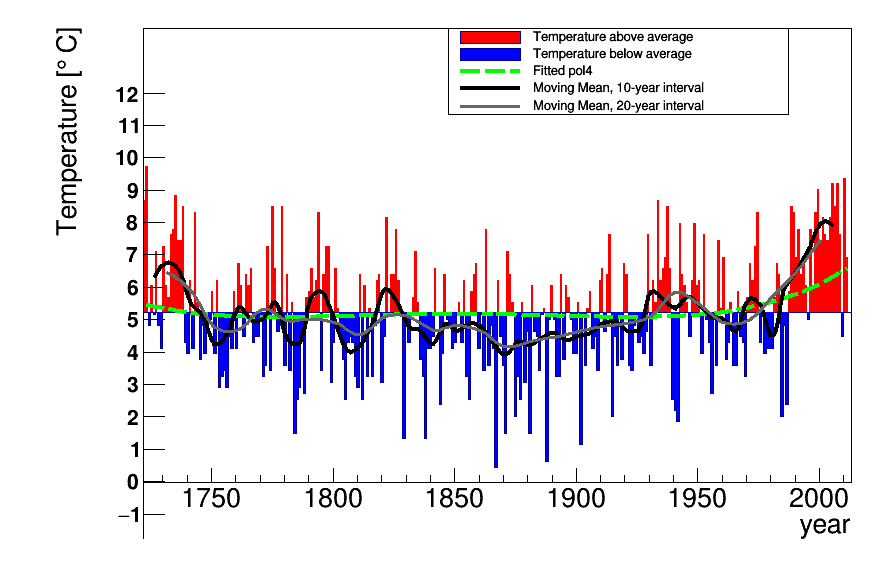
\includegraphics[scale=0.4]{tempYear.png}
    \caption{Histogram showing the annual average temperatures in Uppsala and surroundings from $1722$ to $2013$. The average temperature over the whole period is $5.2$ celsius. Temperatures above this total average are shown in red, those below are shown in blue. A moving-average is shown as the solid green line, and a fit of a polynomial of fourth degree is shown as a black line.}
   \label{fig:year}
\end{figure}
If you use the function t.tempPerYear(2050) it gives you an extrapolated value of over 7 degrees Celsius.

\subsection{Part B:}

\subsection{Part C:}
\begin{enumerate}
\item Q1
\item Q2
\item The warmest and coldest day of each year
\begin{figure}[H]
    \centering
    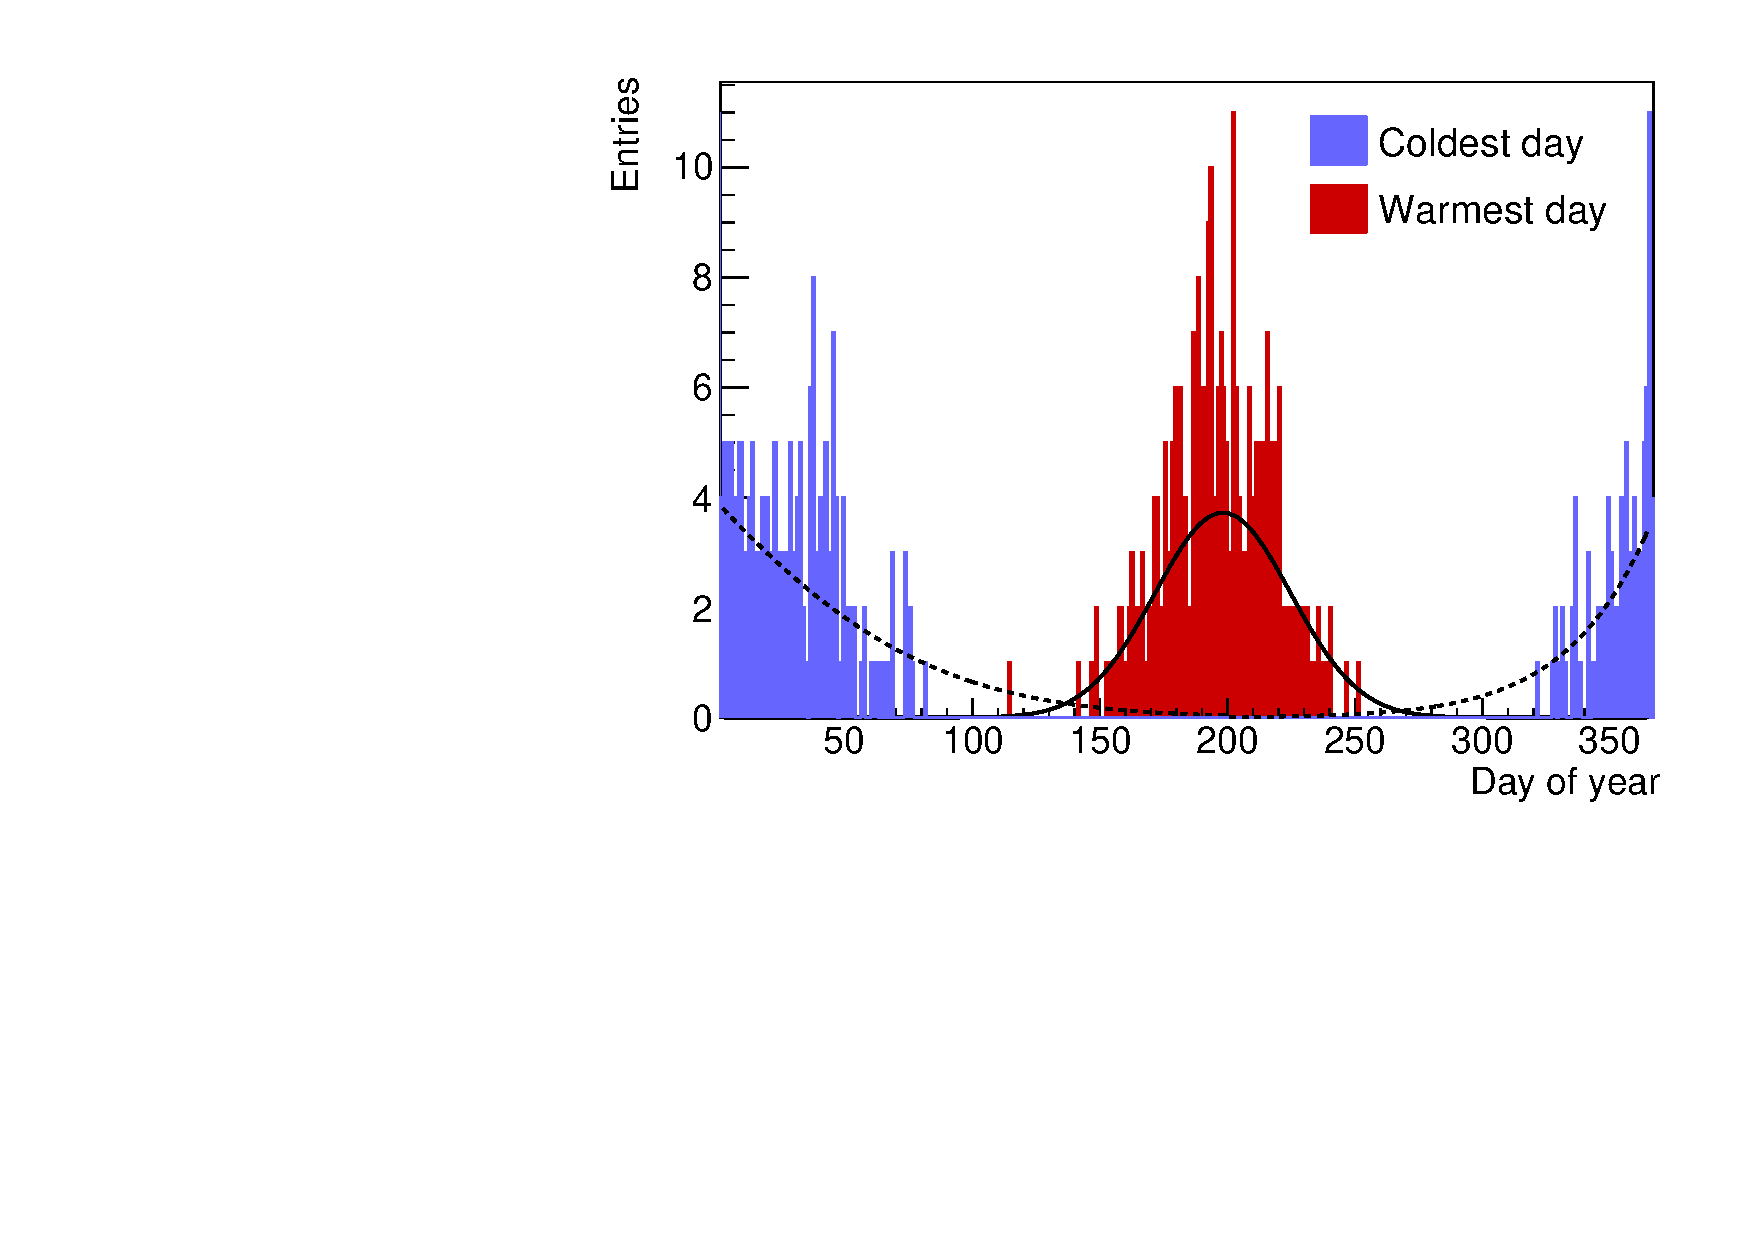
\includegraphics[width=8cm]{./images/hotCold_Upp_final}
    \caption{final histogram}
    \label{fig:hist}
\end{figure}
As the histogram shows, the most likely coldest day is on the end of the year (31/12), and the most likely hottest day is on 13/7.

\end{enumerate}

\section{Discussion}
\subsection{Part A: The rising temperature in Uppsala and surroundings}
From Fig. \ref{fig:year} it is clear that the average temperature is rising not only globally, but also on a local level in mid-Sweden, here we have demonstrated that using measurements from Uppsala and surroundings, but it would be interesting to compare with data from other places around the world, to see how the changes correlate. This is left for future research.

\subsection{Part B:}
\subsection{Part C:}
\begin{enumerate}

\item Q1
\item Q2
\item The warmest and coldest day of each year

The question is to try to find out the possibilites of dates to become the hottest and coldest date. We read the data of Uppsala and then plot the histogram of the occurence for each date being hottest or coldest. 

\begin{figure}[htp]
    \centering
    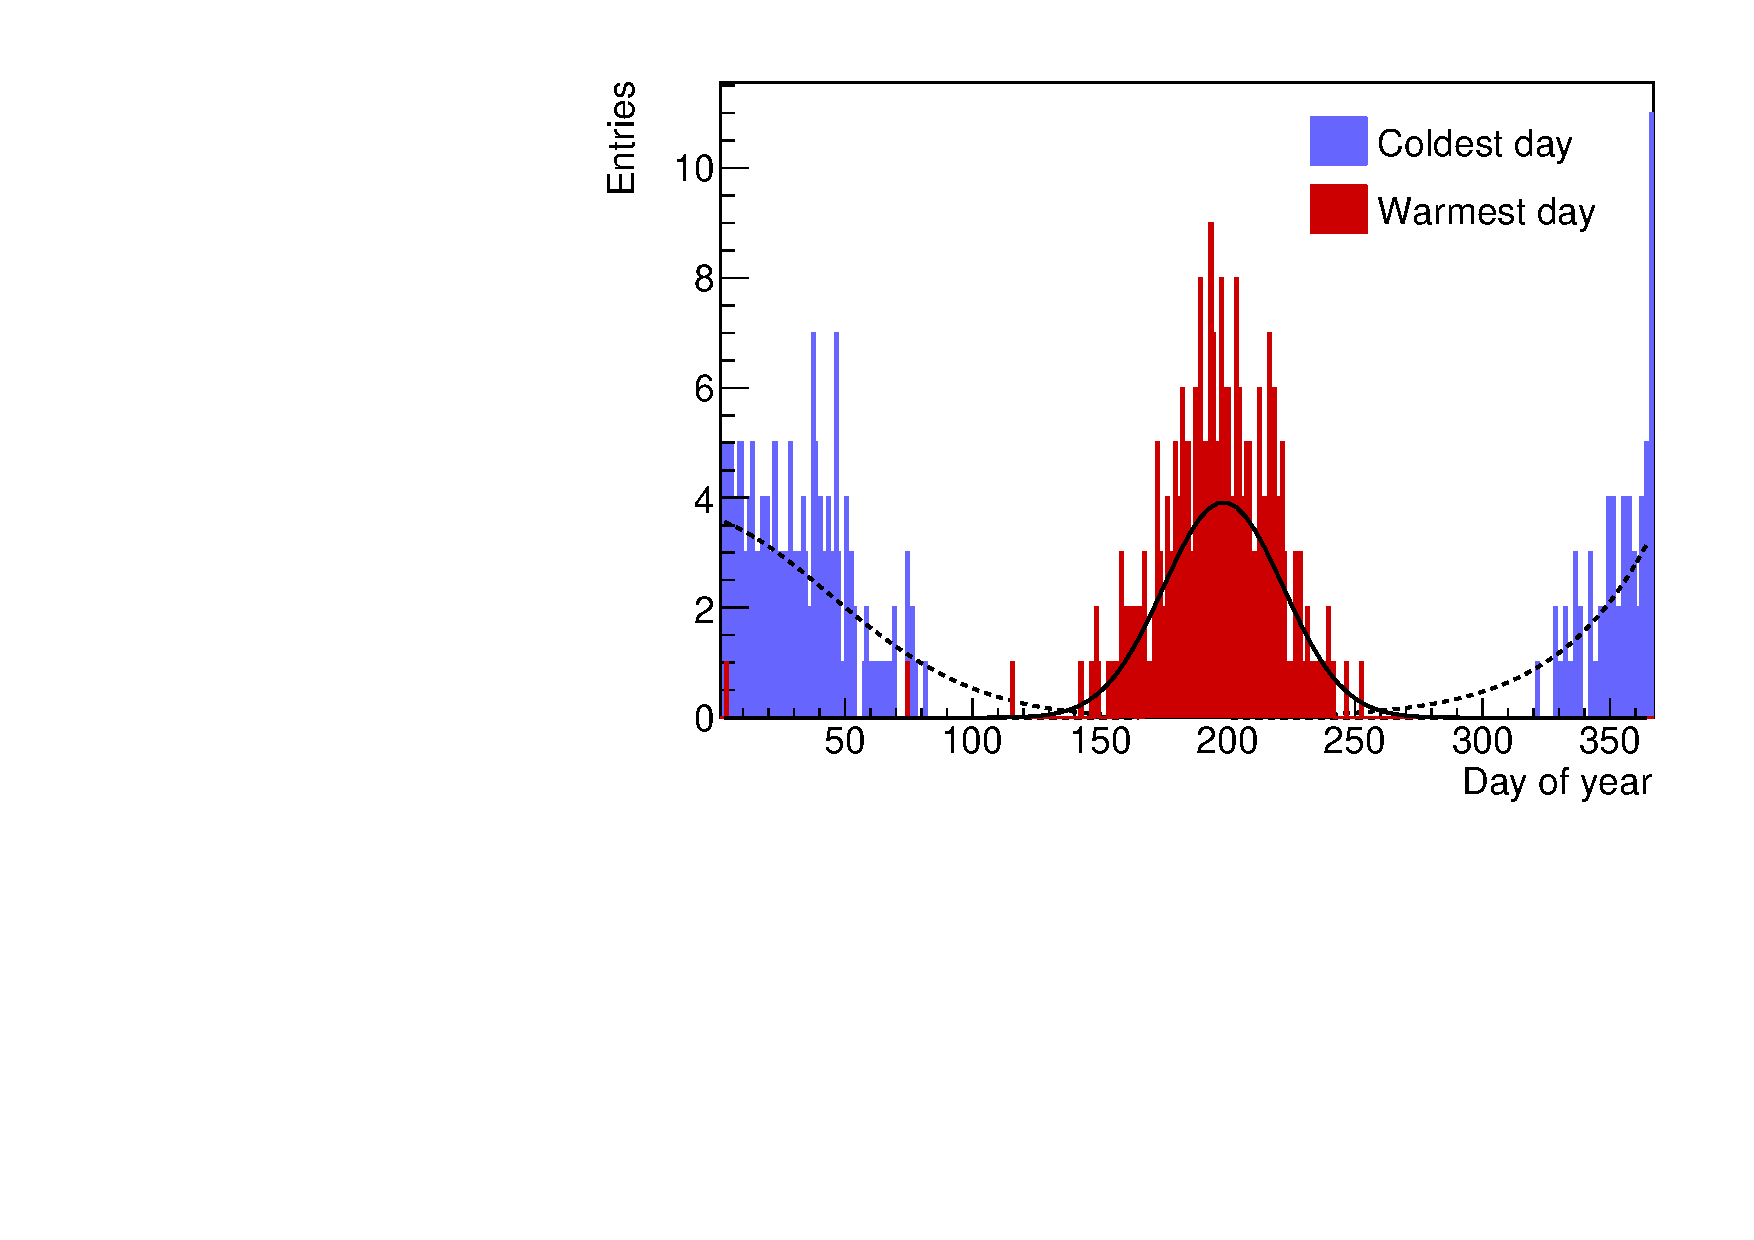
\includegraphics[width=8cm]{./images/hotCold_Upp_prev}
    \caption{first histogram}
    \label{fig:hist}
\end{figure}

We noticed some problem:
\begin{enumerate}
\item There are some coldest date in summer, and also some hottest date in winter, which isn't make sense.
\item Winter is distributed at the first and the end of the year, so we use two Gaussian function to fit on those two parts. However, the plot should be circular in practice. We should take both parts into consideration when we draw fit line.
\end{enumerate}
Then we figured out the cause of the first problem. Because the Uppsala dataset is a combination of some places around Uppsala. For this question, we ignored those places other than Uppsala. This makes the data became uncomplete. For example, data of 1766 are all from Stockholm after April 5, thus the hottest date in 1766 would be April 4, which does not make sense. To solve this, we only accep coldest days which is less than 100 or more than 300 in day of the year, and hottest days which is between 100 and 300 in day of the year.




The graph from the problem where we calculated the nummber of days that had average temperature bellow 0 clearly shows some anomaly in the first few point. It has to do with bad data. The cvs file denoted the quality of the with G for good and bad with Y 



To solve the second problem, we extend the length of the x-axis of histogram to 732, twice of a year. Then we just copy the tail to the front, and also the front to the tail. We plot two Gaussian fit lines for coldest date, one at the front and the other one at the end, and these line must be the same. By doing so, we can take all the coldest date into consideration. Finally, we just need to combine all the fit lines in same plot, and only take from day 1 to day 366 and ignore others.
\begin{figure}[htp]
    \centering
    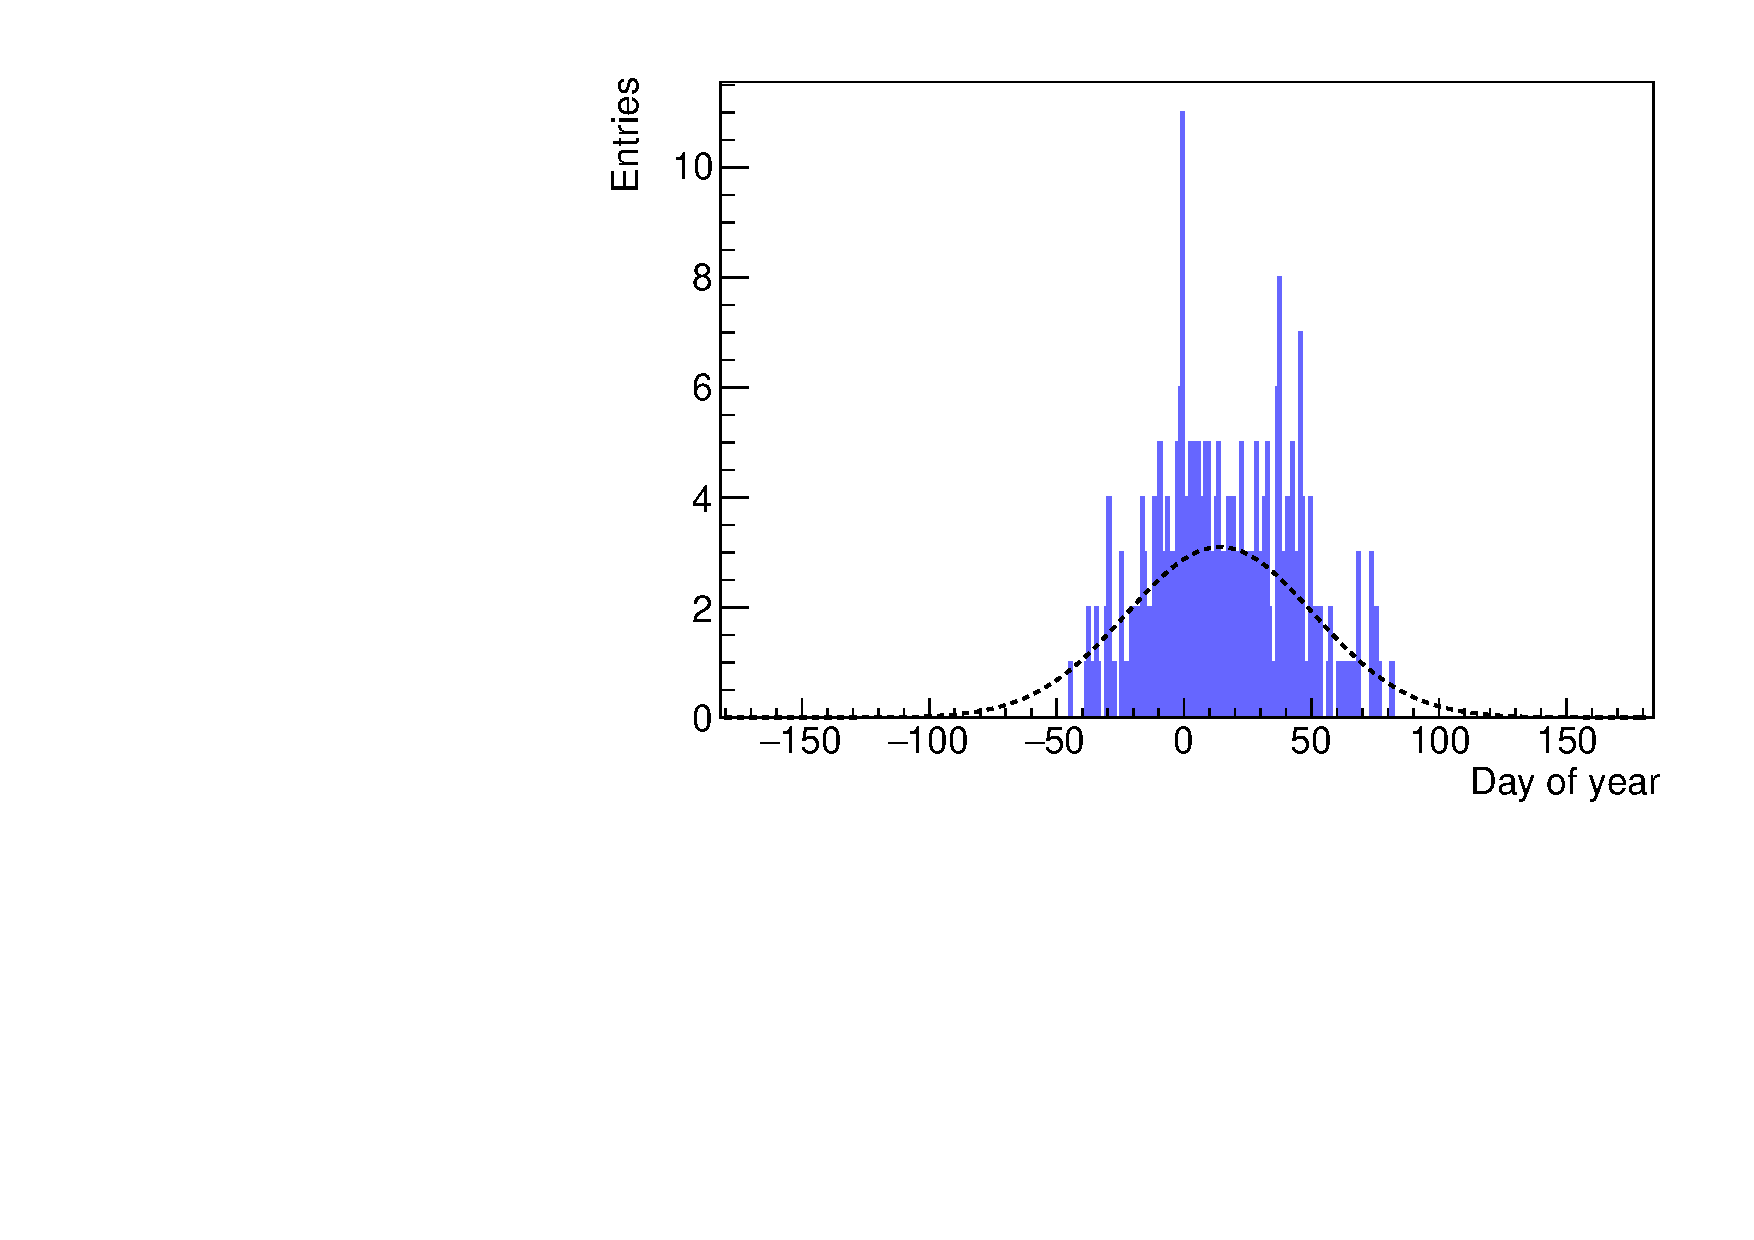
\includegraphics[width=8cm]{./images/hotCold_Upp_cold_1}
    \caption{extended histogram at the begin of the year}
    \label{fig:hist}
\end{figure}
\begin{figure}[htp]
    \centering
    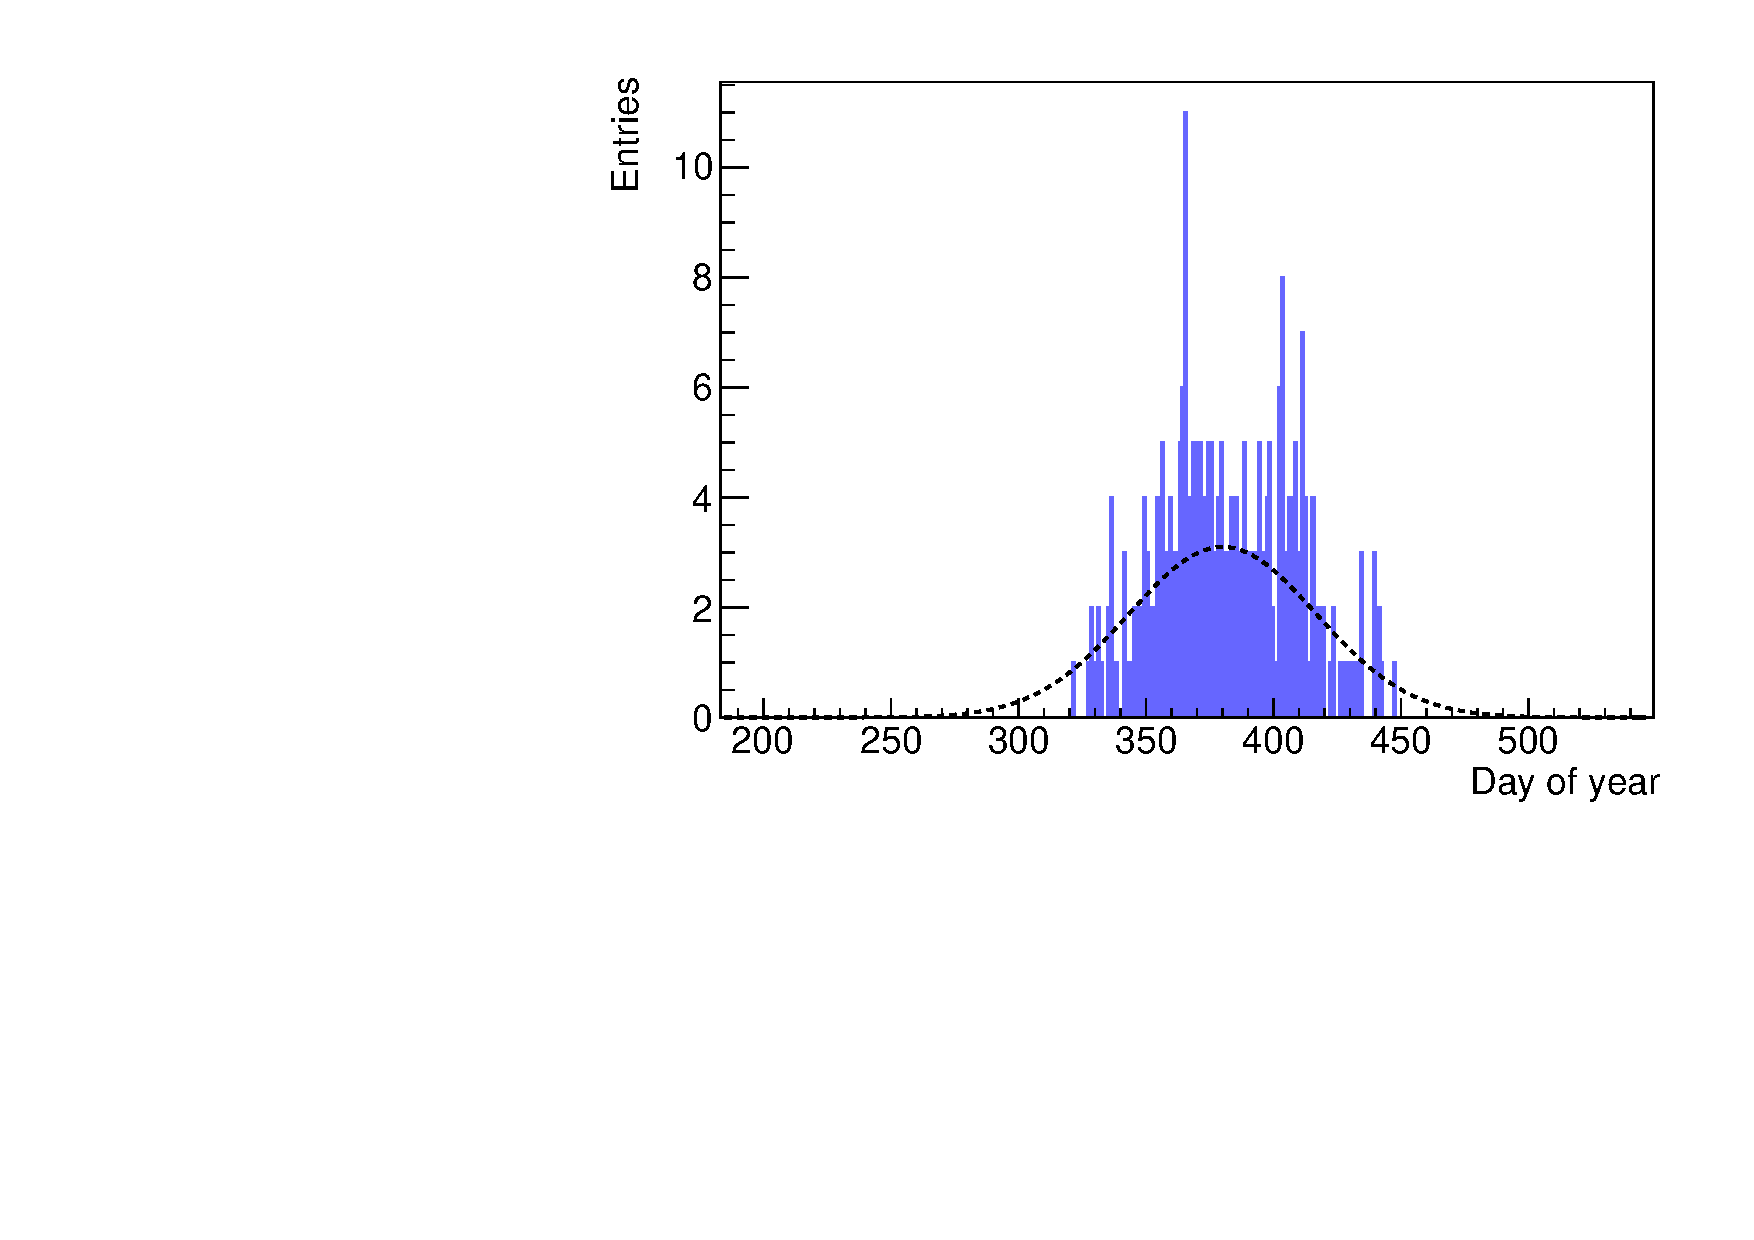
\includegraphics[width=8cm]{./images/hotCold_Upp_cold_2}
    \caption{extended histogram at the end of the year}
    \label{fig:hist}
\end{figure}

The final histogram:
\begin{figure}[htp]
    \centering
    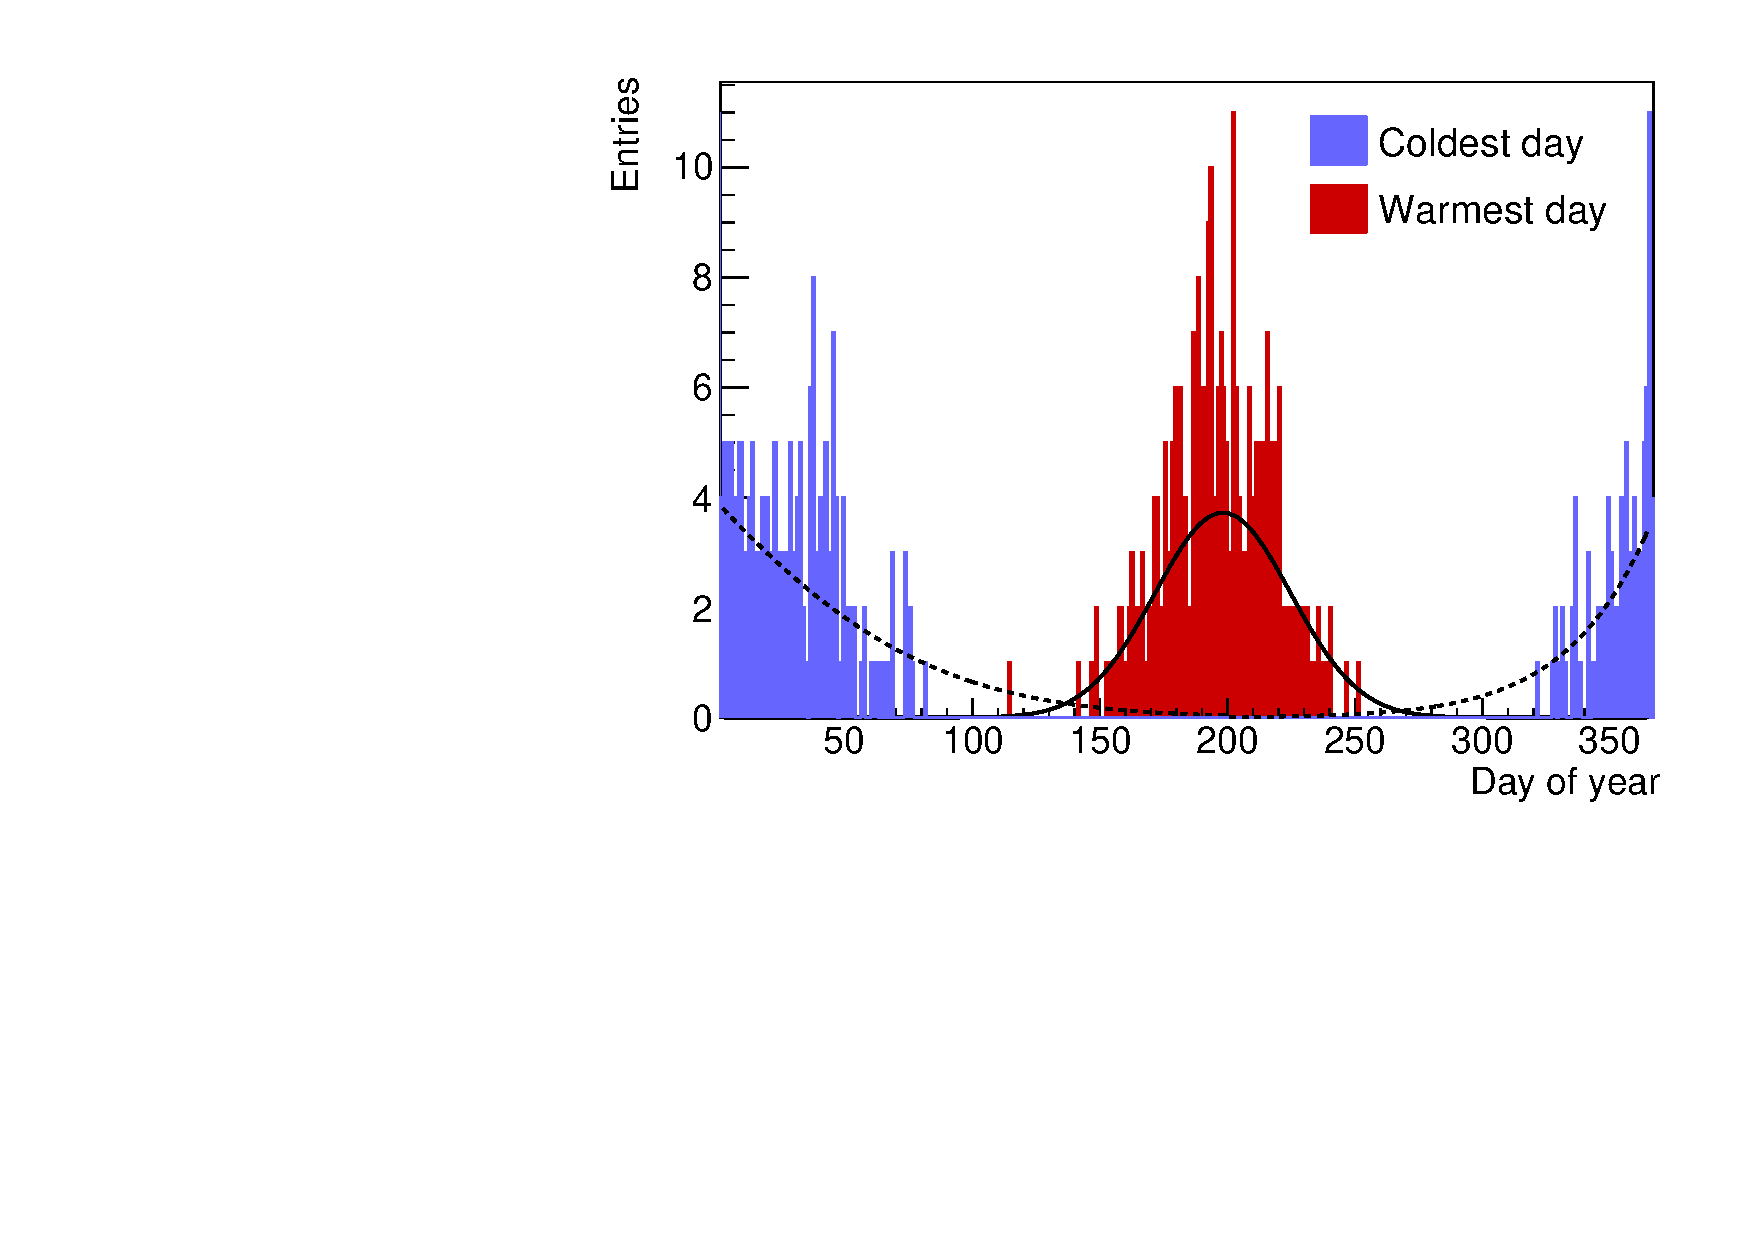
\includegraphics[width=8cm]{./images/hotCold_Upp_final}
    \caption{final histogram}
    \label{fig:hist}
\end{figure}
\end{enumerate}




\end{document}

    © 2019 GitHub, Inc.
    Terms
    Privacy
    Security
    Status
    Help

    Contact GitHub
    Pricing
    API
    Training
    Blog
    About

